%\section*{Background}
%\label{sec:background}

% maybe be clear about how dnaa does not depend on ctra
% stability of CtrA~P itself not just associated with CpdR degradation pathway
% ccka acts as a phosphatase when bound to c-di-GMP
% divk inhibits divl sentence/
% pled localization more important than thought because if present at new pole the sequestration mechanism of divk via plec doesn't make sense

\textit{Caulobacter crescentus} is a free-living (i.e. non-parasitic) \textit{alphaproteobacterium}, which is a gram negative class of bacteria, and is found in fresh water environments~\cite{collier2016}.
\textit{C. crescentus} has an asymmetric cell cycle, a property that is common in this class of bacteria, with a swarmer cells and stalked cells (\cref{fig:cell-cycle-overview}).
The labels of the cell cycle phase are taken from those used for eukaryotes, with a G1, S, and G2 phase.
The swarmer cells (G1 phase) are motile, with a flagellum, pili, and chemotaxis machinery, and are unable to initiate DNA replication.
The stalked cells are permanently stationary (S and G2 phases), held to a surface by a holdfast on the end of a stalk, and initiate DNA replication upon transformation to this cell type.
The transition from the swarmer to stalked phase is regulated on multiple levels, with inputs including the nutritional state of the environment, proximity to a surface, the time spent in the swarmer phase, and even the presence blue light~\cite{berne2019,fiebig2014,purcell2007}.
A stalked cell will always divide into another stalked cell and a swarmer cell.
Unlike many other bacteria, DNA replication initiation only occurs once per cell cycle.
    
\begin{figure}
    \centering
    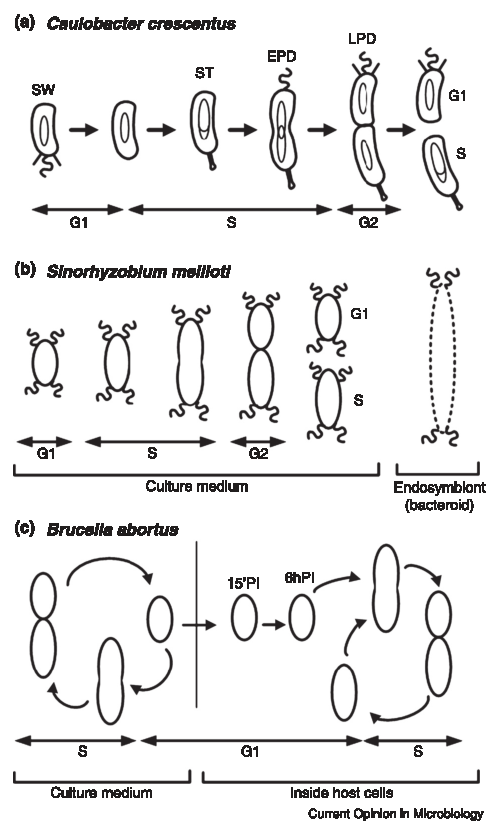
\includegraphics{cell-cycle-overview}
    \caption{
        Overview of the asymmetric cell cycle of \textit{C. crescentus} and two other \textit{alphaproteobacteria}.
        SW: swarmer, ST: stalked, EPD: early-predivisional, LPD: late-predivisional.
        From~\cite{collier2016}.
        \label{fig:cell-cycle-overview}
     }
\end{figure}

%\section*{The cell cycle is controlled by master regulators} 
%\label{sec:master-regulators}

Seven master regulators, CtrA, GcrA, DnaA, SciP, MucR1, MucR2, and CcrM, control the cell cycle in a cascading fashion, with oscillations in their concentration and activity controlled by their promotion and suppression of each other and through signalling pathways taking inputs from the metabolic state and the environment~\cite{lasker2016}.
CcrM is a DNA methyltransferase, while the rest are transcription factors.
Nearly a third of the genes in \textit{C. crescentus} are cell cycle-regulated, with half under the direct control of at least one of these master regulators, and another half of those being controlled in a combinatorial manner by more than one of these master regulators (\cref{fig:cell-cycle-genes}).
\Cref{fig:master-regulators} gives an overview of how the master regulators interact with each other and some of the major cell modules, and when they are present and active in the cell cycle.
GcrA and CcrM have regulons (i.e. the set of genes under their transcriptional control) that overlap substantially, and GcrA activity is modulated by the CcrM dependent methylation of the promoter \cite{mouammine2018}.
The picture can be simplified somewhat by ignoring both of these regulators, given that \textcite{murray2013} found that both genes could be deleted without loss of viability; they speculate these regulators act to increase robustness.
MucR1/2 and SciP inhibit genes activated by CtrA in particular parts of the cell cycle, with SciP acting in the G1 phase and MucR1/2 acting in the G2 phase \cite{collier2016,fumeaux2014}.
Perhaps the two most fundamental regulators then are DnaA and CtrA.

\begin{figure}
    \centering
    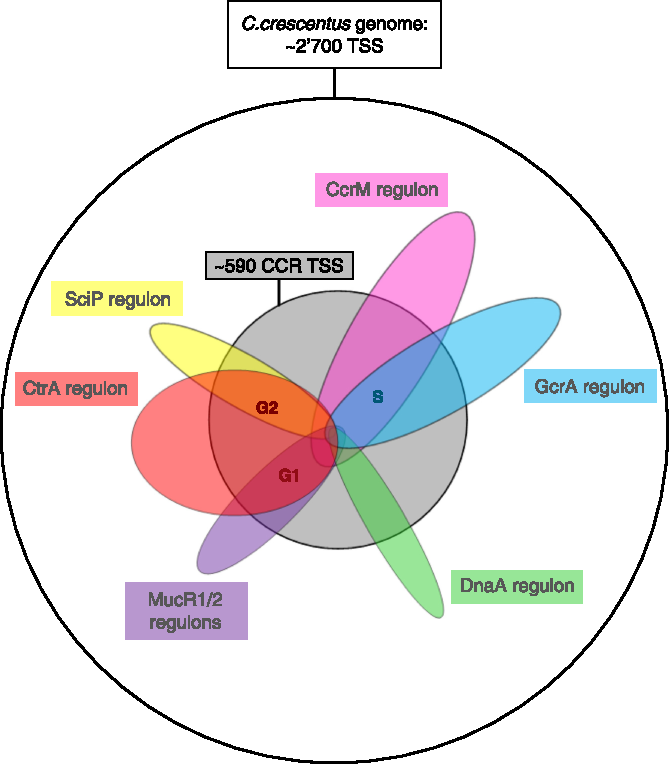
\includegraphics{cell-cycle-genes}
    \caption{
        Many genes in \textit{C. crescentus} are cell-cycle regulated.
        CCR TSS: cell cycle regulated transcription start sites.
        From~\cite{collier2016}.
        \label{fig:cell-cycle-genes}
     }
\end{figure}
    
\begin{figure}
    \centering
    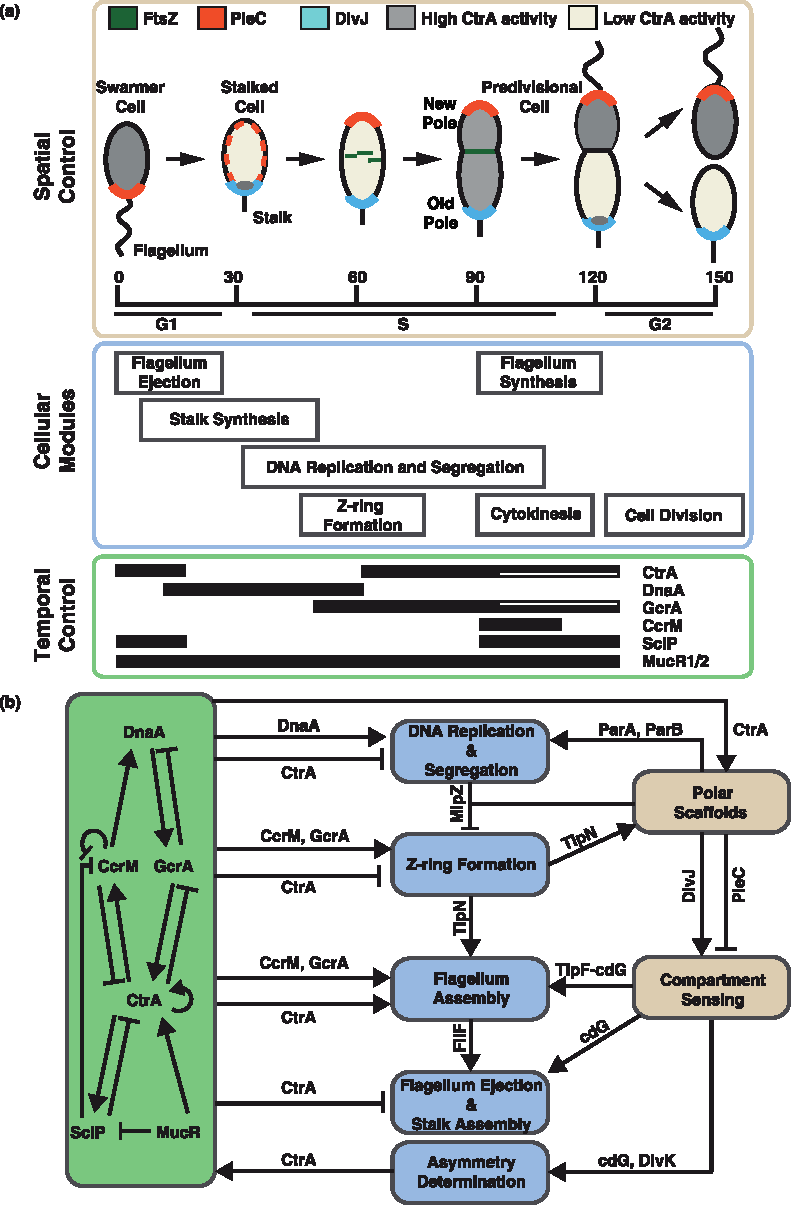
\includegraphics{master-regulators}
    \caption{
        Master regulators across the cell cycle and their interactions with each other and cell modules.
        Note that while MucR1/R2 is not under transcriptional control of the others and does not have oscillations in its concentration, it its activity is controlled post-translationally.
        From~\cite{lasker2016}.
        \label{fig:master-regulators}
     }
\end{figure}

The origin of replication (often referred to as the Cori, for \textit{Caulobacter} ori) has multiple binding sites for DnaA and CtrA, with some overlap~\cite{frandi2019}.
As in other classes of bacteria, DnaA binds to the Cori to initiate DNA replication.
However, if CtrA is bound to the Cori it blocks DnaA binding and thus the initiation of replication.
The spatial and temporal control for CtrA is key to \textit{C. crescentus}'s assymetric cell cycle in which swarmer cells are unable to replicated their DNA.
The basic roles of DnaA and CtraA and how they functionally interact are perhaps best illustrated by the work of \textcite{jonas2011} in \cref{fig:ctra-dnaa}.
When both are present, DNA replication is initiated once per cell cycle, immediately following division in the stalked cell.
When CtrA is knocked out, the cell never divides, but replication is initiated with the same frequency.
When DnaA activity is increased, DNA replication occurs multiple times in the same cycle.
When DnaA activity is decreased but not eliminated, the period of DNA replication initiation is increased, but only marginally, indicating that fine control over DnaA levels is likely not required for cell cycle timing.
DnaA levels were found to vary by only a factor of two over the cell cycle~\cite{felletti2019}.

\begin{figure}
    \centering
    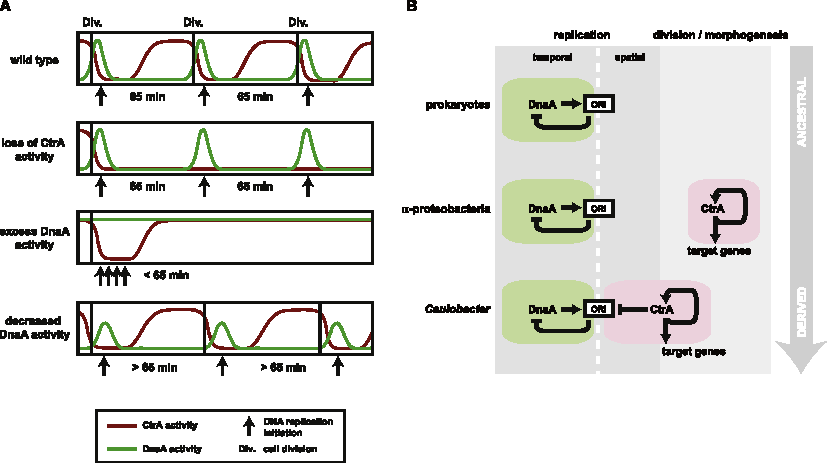
\includegraphics{ctra-dnaa}
    \caption{
        CtrA and DnaA activity levels over the cell cycle of a stalked cell, with division and replication events indicated with a line and an arrow, respectively.
        On the right is a cartoon showing how the coupling between DNA replication and cell division has evolved.
        From~\cite{jonas2011}.
        \label{fig:ctra-dnaa}
     }
\end{figure}

Aside from being regulated transcriptionally, CtrA activity is regulated post-translationally by phosphorylation and proteolysis (\cref{fig:ctra-regulation}).
When CtrA is phosphorylated it is active and stabilized to degradation~\cite{frandi2019}.
The key protein which controls the activity of CtrA is CckA.
CckA acts as a kinase of ChpT when bound to cyclic diguanylate (c-di-GMP), and a phosphatase otherwise.
ChpT transfers the phosphate group between itself and either CtrA or another protein, CpdR.
CpdR, when not phosphorylated, binds to RcdA, PopA, and ClpX, which leads to degradation of CtrA.
c-di-GMP levels increase during the G1 to S phase transition~\cite{hallez2017}, thus leading to a reduction in CtrA activity, and afterwards decrease.
The c-di-GMP levels themselves are controlled by PleD and PdeA.
The presence of PdeA seems to keep ci-di-GMP levels lows, and is itself degraded by CpdR and upregulated by CtrA.
PleD is a c-di-GMP synthase whose activity is controlled post-translationally by its phosphorylation state, which will be discussed shortly.

\begin{figure}
    \centering
    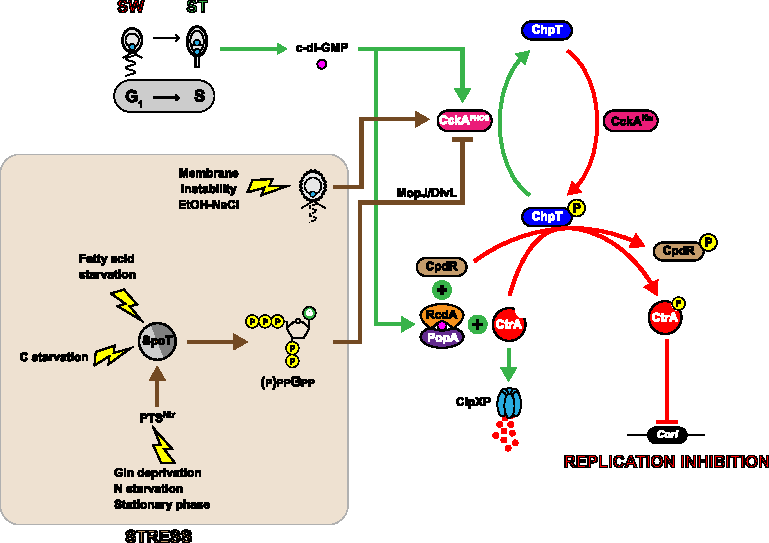
\includegraphics{ctra-regulation}
    \caption{
        The regulation of CtrA.
        From~\cite{frandi2019}.
        \label{fig:ctra-regulation}
     }
\end{figure}

It is known that DnaA levels fluctuate over the cell cycle, but the factors that control the transcriptional and translational regulation are still unknown.
There is some evidence that small non-coding RNAs (sncRNAs) may be involved in cell cycle and environment response regulation of DnaA translation~\cite{felletti2019}.
However, regulation of the concentration of DnaA does not appear to be necessary for its role in regulating DNA replication initiation~\cite{jonas2011}.
Instead, as in other classes of bacteria, DnaA binds ATP and has ATPase activity, and only DnaA-ATP is able to initiate DNA replication (\cref{fig:dnaa-regulation}).
The well characterized RIDA (regulatory inactivation of DnaA) mechanism ensures that DNA replication does not occur multiple times after DNA-ATP levels are high enough.
RIDA involves a protein recruited to the replisome, HdaA, stimulating DnaA ATPase activity.
In addition to this, DnaA-ADP is specifically degraded by a protease, Lon.

\begin{figure}
    \centering
    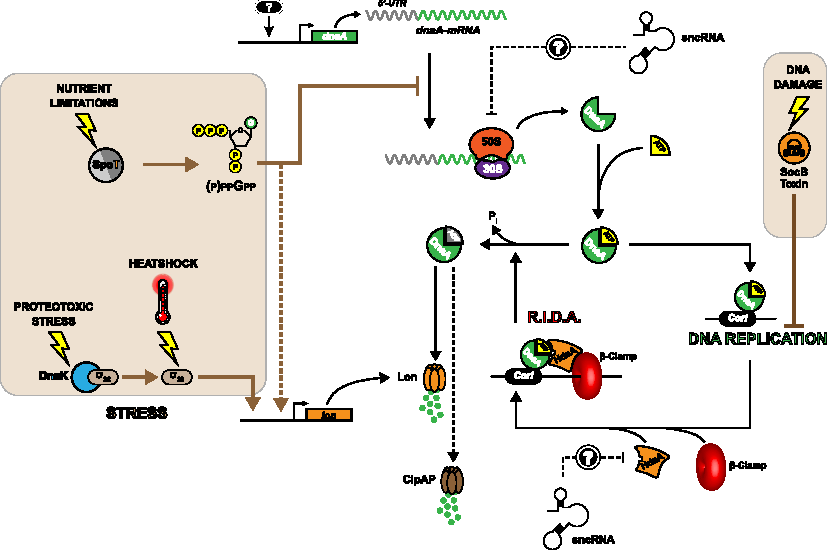
\includegraphics{dnaa-regulation}
    \caption{
        The regulation of DnaA.
        From~\cite{frandi2019}.
        \label{fig:dnaa-regulation}
     }
\end{figure}

Cell division is also controlled at multiple levels.
MipZ is a protein that inhibits the polymerization of FtsZ and plays a role similar to MinD in \textit{E. coli}~\cite{collier2019}.
It binds to other proteins which bind to the chromosome near the Cori; in swarmer cells, the Cori is localized to the flagellar pole.
After the swarmer-to-stalked transition, upon initiation of replication, the new Cori migrates to the opposite cell pole.
This results in the concentration of MipZ being lowest in the middle of the cell, allowing for formation of the Z-ring.
Both ftsZ and mipZ are activated by both DnaA and GcrA and repressed by CtrA, allowing them to be upregulated during the S-phase and downregulated afterward.
Genes that encode proteins that are recruited later to the divisome are activated by CtrA but repressed by SciP, allowing them to be upregulated later in the S-phase, after the Z-ring has formed.
The divisome proteins are relatively susceptible to degradation by proteases, which allows these master regulators to have maximal effect on the timing of their levels~\cite{collier2019}.

Regulation of the cell cycle is also linked to nutrient conditions and cell metabolism.
In nutrient poor conditions, guanosine tetra- or penta-phosphate ((p)ppGpp) is produced, which increases the CtrA activity and decreases DnaA activity and leads to the cessation of chromosome replication~\cite{frandi2019}.
It does this by inhibiting CckA phophatase through a pathway involving the proteins MopJ and DivL, which increases the stability of CtrA by allowing it to remain phosphorylated (\cref{fig:ctra-regulation}), and by inhibiting DnaA translation (in a manner not fully understood), leading to the clearance of DnaA by proteolysis (\cref{fig:dnaa-regulation}).
To be clear, while changes in the total concentration of DnaA are not important in the regulation of DNA initiation under good growth conditions, changing the total concentration of DnaA is used to regulate DNA initiation under poor nutrient conditions, rather than only changing the ratio of DnaA-ATP to Dna-ADP.

Cell division is also sensitive to changes in nutrient conditions, with downregulation of ftsZ and mipZ occurring when nitrogen levels are low~\cite{collier2019} (\cref{fig:cell-division-metabolism}).
FtsZ polymerization is also inhibited by a protein, GdhZ, that converts glutamate to an intermediate in TCA cycle in the presence of NAD.
The inhibition of FtsZ polymerization can only occur when the metabolic substrates are present, which results in it only acting in the G1 and G2 phases, apparently to prevent Z-ring formation in swarmer cells and possibly to assist in triggering constriction of the Z-ring in pre-divisional cells.
The effect is amplified by the binding of a side-product of the GdhZ catalyzed reaction, NADH, to another protein which then further inhibits Z-ring formation.
The central metabolism is also connected to peptidoglycan synthesis through the same intermediate in the molecule in the TCA cycle, and since cell wall synthesis is a key part of cell division, it may provide another channel by which nutrient conditions can lead to regulation of the cell cycle~\cite{collier2019}.

\begin{figure}
    \centering
    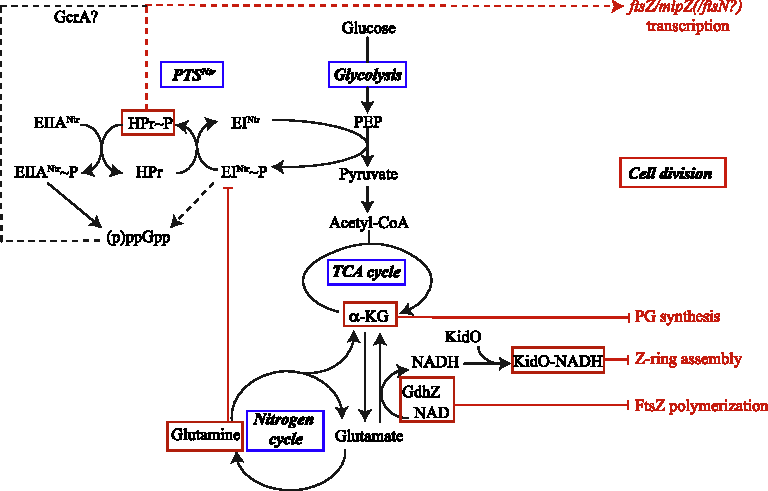
\includegraphics{cell-division-metabolism}
    \caption{
        Links between metabolism and cell division.
        From~\cite{collier2019}.
        \label{fig:cell-division-metabolism}
     }
\end{figure}

The organization of proteins at the poles is key to maintaining an asymmetric cell cycle.
In a swarmer cell, the flagellar pole is the old the pole, which becomes the stalked pole upon transition to a stalked cell.
The poles have a different set of proteins and activities associated with them.
There is a complex hierarchy of interactions in which proteins are recruited to the poles that is not fully understood.
When the cell divides, the new pole is marked by the presence of TipN, which is localized from the previous new pole by the Z-ring during cell division~\cite{lasker2016}.
The old pole in a swarmer cell is marked by a scaffolding protein, PopZ.
Upon transitioning to a stalked cell, PopZ eventually forms a second locus at the new pole.
The transition is not fully understood but appears to be a Turing pattern formed by a reaction-diffusion mechanism~\cite{subramanian2017}.
PopZ interacts with the Cori through Par proteins and is involved in anchoring the Cori to the old pole in the swarmer cell.

The spatiotemporal regulation of flagellum and pilli ejection and holdfast and stalk synthesis at the old pole, flagellum and pilli synthesis at the new pole, and differentiation of the swarmer and stalked cell at cell division involves a complex set of interactions.
These involve two proteins that can act as either phosphatases or kinases, CckA (previously discussed) and PleC, two other kinases, DivJ and DivL, and two response regulator, the above discussed master regulator CtrA and DivK, the above mentioned pole markers, and further pole scaffold proteins, SpmX and PodJ.
DivK can interact with PleC to convert it to a kinase, and has a higher affinity for PleC in its phophatase mode when it itself is phosphorylated~\cite{subramanian2017}.
DivK can also enhance the kinase activity of DivJ~\cite{kirkpatrick2012}.
DivJ acts to phosphorylate DivK while PleC itself acts on DivK to dephosrylate it.
Altogether, these feedback loops result in bistability that allows a switch like response in the activity state of PleC to the change in local DivJ concentrations~\cite{subramanian2017}.

\Cref{fig:spatiotemporal-distribution} gives the distributions of these proteins as a function of their position along the cell length and time in the cell cycle as calculated in the model of \textcite{subramanian2015}, while \cref{fig:polar-localization} summarizes this into a cartoon.
At the transition to a stalked cell, DivJ localizes to the old pole through a mechanism not yet determined, but which seems to involve a SpmX, which itself interacts with PopZ~\cite{kirkpatrick2012}.
PleC in its kinase state then phosphorylates PleD, which, through mechanisms not fully understood, lead to the ejection of the flagellum and pilli and synthesis of the stalk.
PleC, through a mechanism not fully understood, although involving PodJ and possibly TipN, delocalizes from the old pole and eventually relocalizes to the new pole.

\begin{figure}
    \centering
    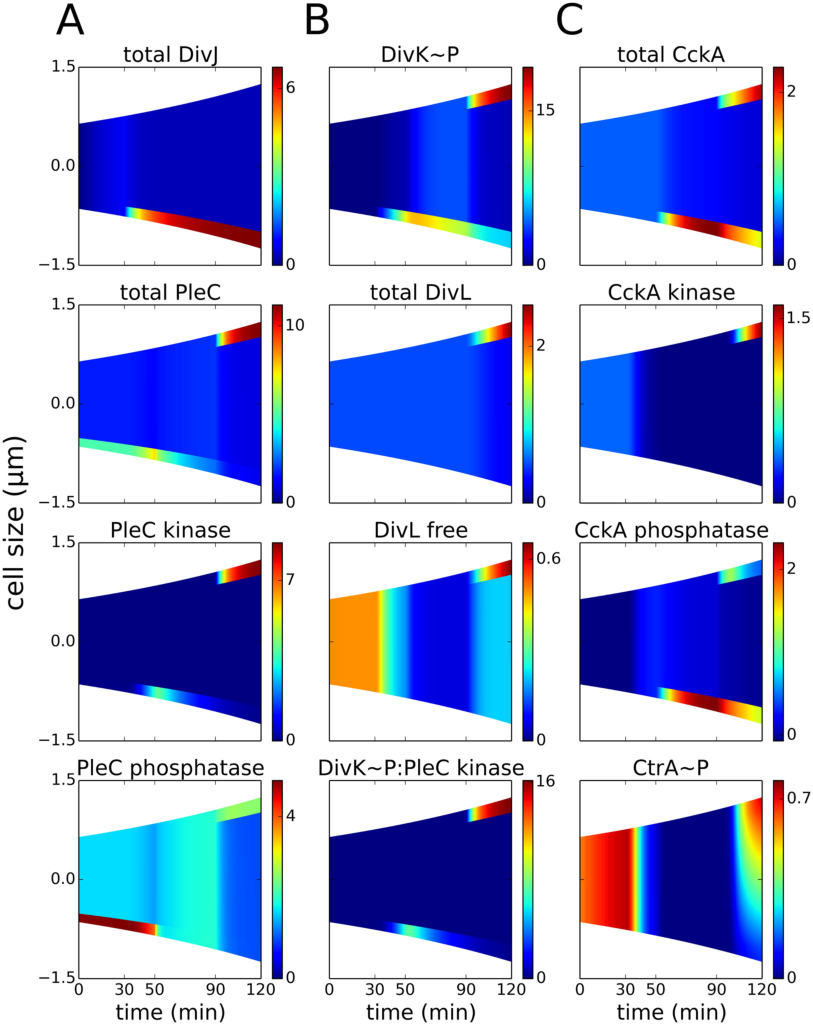
\includegraphics{spatiotemporal-distribution}
    \caption{
        Spatiotemporal distribution of proteins over the cell cycle form a deterministic reaction diffusion model, starting from a swarmer cell and ending before cell division.
        From~\cite{subramanian2015}.
        \label{fig:spatiotemporal-distribution}
     }
\end{figure}

\begin{figure}
    \centering
    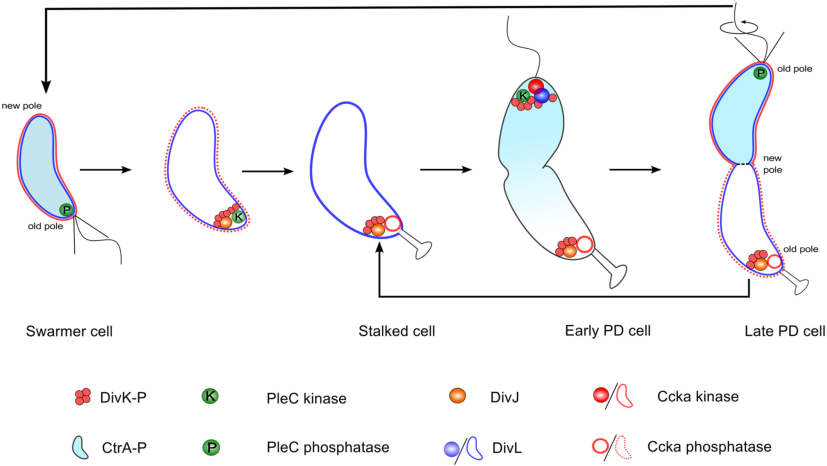
\includegraphics{polar-localization}
    \caption{
        Localization of asymmetry determining proteins.
        From~\cite{subramanian2015}.
        \label{fig:polar-localization}
     }
\end{figure}

A gradient of phosphorylated CtrA is formed in the predivisional cell, which leads to sequestration of more CtrA in the swarmer cell.
This gradient is formed by the localization of CckA to the poles through an interaction with PopZ, and by CckA acting as a kinase at the new pole and a phosphatase at the old pole.
The differential CckA activity means that after the lipid bilayer fissions, the to-be swarmer cell compartment continues to increase its CtrA levels, while the remaining CtrA in the to-be stalked cell compartment is degraded.
DivL is inhibited by phosphorylated DivK, while DivL acts to convert CckA to a kinase.
DivL, like PleC, is localized to the new pole in pre-divisional cells with some mechanism involving PodJ.
While phosphorylated DivK is also localized to the new pole in predivisional cells, modeling suggests that it is sequestered away from DivL in a complex with PleC, allowing DivL to act on CckA.

By following single cells across multiple generations, it was determined that \textit{C. crescentus} cells grow exponentially and divide once they reach a multiple of their initial size (1.8), and that the mean division time is proportional to the inverse of the mean growth rate~\cite{iyer-biswas2014}.
Building on this work and a further study developing methods for measuring the dimensions of individual cells~\cite{wright2015}, \textcite{banerjee2017} developed a phenomenological model of the size regulation.
They find the data best fit a mixer model, which combines a timer model, where the final size is proportional to the initial size and the interdivision time is constant, and an adder model, where the final size is the initial size plus a constant and the interdivision time decreases with increasing cell size.
By measuring the minimum width of the cells, they determined that there was a slow and a fast constriction phase, and that the slow constriction phase corresponded to the timer component of the model, and the fast constriction phase to the adder component.
Here the timer component is a relative one, with the crossover time between slow and fast constriction being controlled by the growth rate and constant when normalized by the interdivision time.
With fluorescent images and a simple model, they determined that in the slow constriction phase the cell wall is added uniformly, while in the adder phase the cell wall is primarily added to the growing septum (\cref{fig:cell-wall-growth}).
The added length in this phase is length of the final septum.
They speculate that the timer phase corresponds to the S-phase, although they do not give any evidence for this or any other molecular mechanism for the size control.
Given that DNA replication is initiated at birth, it seems a reasonable hypothesis.
It is likely that the regulation of the assembly and dynamics of the divisome are involved triggering the crossover from slow to fast constriction.

\begin{figure}
    \centering
    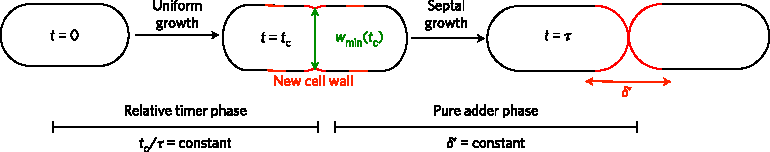
\includegraphics{cell-wall-growth}
    \caption{
        Cell wall growth dynamics.
        From~\cite{banerjee2017}.
        \label{fig:cell-wall-growth}
     }
\end{figure}
